\documentclass{article}

\usepackage[utf8]{inputenc} 
\usepackage[russian]{babel} 
\usepackage{amsmath} 
\usepackage{hyperref} 
\usepackage{graphicx}
\usepackage{amssymb}
\newcommand{\numberset}[1]{\mathbb{#1}} 
\newcommand{\N}{\numberset{N}}
\newcommand{\Q}{\mathbb Q}
\newcommand{\R}{\mathbb R}
\newcommand{\Z}{\mathbb Z}
\usepackage[a4paper, total={6in, 8in}]{geometry}
\usepackage{color}
\usepackage{hyperref}
\hypersetup{
    colorlinks=true,
    linkcolor=blue,
    urlcolor=red,
    linktoc=all
}

\title{Матан экзамен}

\begin{document}
\maketitle 
\tableofcontents
\newpage
\section{БИЛЕТ 24 --  Функция одной вещественной переменной. Области определения и изменения. График функции. Сложная функция. Свойства функции. Обратная функция. Способы задания функции}

Задание \textbf{функции}  $y = f (x)$  вещественной переменной  $x$  означает, что каждому значению  $x$  из числового множества $X$ (области определения) ставится в соответствие число $y$ из числового множества $Y$ (области значений).
\begin{itemize}
    \item \textbf{Аргументом} функции  $y = f (x)$  является вещественная переменная  $x$; аргументом функции  $y = f (x_1, \ldots, x_n)$  является вектор $(x_1, \ldots, x_n)$, составленный из вещественных переменных  $x_1, \ldots, x_n$.
    \item \textbf{Областью определения} функции  $y = f (x)$  является множество  $X$  допустимых значений переменной  $x$. 
    \item \textbf{Областью изменения} функции  $y = f (x)$  является множество  $Y$  допустимых значений переменной  $y$.
\end{itemize}
Пусть функция $u=g(x)$  определена на множестве $X$ и $U$ - множество значений этой функции. Пусть, множество $U$ (или его подмножество) является областью определения функции $y=f(u)$. Поставим  в соответствие каждому $x$ из $X$ число $f(g(x))$. Тем самым на множестве $X$ будет задана функция $y=f(g(x))$. Её называют \textbf{композицией функций} или \textbf{сложной функцией}.
\subsection{Свойства Функций}
Функция называется \textbf{чётной}, если:
\begin{enumerate}
    \item Область определения функции симметрична относительно нуля, т.е. для любого $x$, принадлежащего области определения, $-x$ также принадлежит области определения; 
    \item При замене значения аргумента $x$ нa противоположное $-x$ значение функции не изменится, т.е. $f(-x)=f(x)$ для любого $x$ из области определения функции.
\end{enumerate}
Функция называется \textbf{нечётной}, если
\begin{enumerate}
    \item Область определения функции симметрична относительно нуля, т.е. для любого $x$, принадлежащего области определения, $-x$ также принадлежит области определения; 
    \item $f(-x)=-f(x)$ для любого $x$ из области определения функции.
\end{enumerate}
\subsection{Обратная Функция}
\textbf{Обратная функция} — функция, обращающая зависимость, выражаемую данной функцией. Например, если функция от $x$ даёт $y$, то обратная ей функция от $y$ даёт $x$. Обратная функция функции $f$ обычно обозначается $f^{-1}$.
\subsection{Способы задания функций}
\begin{enumerate}
    \item Табличный способ
    \item Графический способ
    \item Аналитический способ
    \item Словесный способ
\end{enumerate}
\newpage
\section{БИЛЕТ 25 -- Два определения предела функции и их эквивалентность}
\begin{itemize}
    \item Определение предела по Коши 
    $$ \lim_{x\to x_0} f(x)=A\, \Leftrightarrow\,\forall\, U(A)\:\:\exists \, U(x_0)\: :\: f(X\cap U(x_0))\subset U(A) $$
    $$ \lim_{x\to x_0} f(x)=A\Leftrightarrow \,\forall\,\varepsilon\:\:\exists\,\delta>0\:\:\forall \, x\in X\,:\: (|x-x_0|<\delta \Rightarrow \, |f(x)-A|<\varepsilon)  $$
    \item Определение предела по Гейне
    $$ \lim_{x\to x_0} f(x) =A\,\Leftrightarrow\,\forall\, x_n ,\,\lim_{n\to\infty} x_n=A\:\: :\: \lim_{n\to\infty} f(x_n)=A $$
\end{itemize}
\subsection{Эквивалентность определений}
Пусть число $A$ является пределом функции $f(x)$ в точке $a$ по Коши. Выберем произвольную подходящую последовательность $x_n$ , $n \in N$, то есть такую, для которой $\lim\limits_{n\rightarrow \infty } x_n = a$. Покажем, что $A$ является пределом по Гейне.
\newline
Зададим произвольное $\varepsilon > 0$ и укажем для него такое $\delta > 0$, что для всех $x$ из условия $0 < |x-a| < \delta$ следует неравенство $|f(x)-A | < \varepsilon$. В силу того, что $\lim\limits_{n\rightarrow \infty } x_n = a$, для $\delta > 0$ найдётся такой номер $n_{\delta }\in N$, что $\forall n\geqslant n_{\delta }$ будет выполняться неравенство $|f(x_{n})-A| < \varepsilon$, то есть $\lim\limits_{n\rightarrow \infty } f(x_{n}) = A$.
\newline
Докажем теперь обратное утверждение: предположим, что $\lim\limits_{x\rightarrow a } f(x) = A$ по Гейне, и покажем, что число A является пределом функции $f(x)$ в точке $a$ по Коши. Предположим, что это неверно, то есть: $\exists\: \varepsilon_{0} > 0\: \forall\, \delta > 0 \::\:\exists\: x_{\delta }:0<|x_{\delta }-a|<\delta \Rightarrow |f(x_{\delta })-A|\geqslant \varepsilon$. В качестве $\delta$ рассмотрим $\delta = \frac{1}{n}$, а соответствующие значения $x_{\delta }$ будем обозначать $x_{n}$. Тогда при любом $n\in N$ выполняются условия $|x_{n}-a|<\frac{1}{n}$ и $|f(x_{n})- A | \geqslant \varepsilon$. Отсюда следует, что последовательность $x_{n}$ является подходящей, но число $A$ не является пределом функции $f(x)$ в точке $a$. Получили противоречие.
\newpage
\section{БИЛЕТ 26 -- Бесконечные пределы и односторонние пределы}
Функция имеет \textbf{бесконечный} предел, если
$$ \lim_{x\to a} f(x) = + \infty\: (-\infty)\, \Leftrightarrow \, \forall\, M>0\:\:\exists\,\delta >0\:\::\:\:\forall x\in X, \,|x-a|<\delta\:\:: \: f(x)>M\:\:(f(x)<-M)$$
Число $A$ называется \textbf{левосторонним} пределом, если
$$ \lim_{x\to a-0} f(x)=A\,\Leftrightarrow\,\forall\,\varepsilon>0\:\: \exists\,\delta >0\:\: :\:\:\forall x \in X,\, a-x<\delta\:\: :\: |f(x)-A|<\varepsilon$$
\newpage
\section{БИЛЕТ 27 -- Свойства пределов функции. Ограниченность функции, имеющей предел. Предельный переход в неравенстве. Теорема о сжатой переменной. Отделимость от нуля}
\subsection{Свойства пределов функций}
\begin{itemize}
    \item \textbf{ТЕОРЕМА ОБ ОТДЕЛИМОСТИ ОТ НУЛЯ} Если функция имеет конечный предел в точке, то существует окрестность этой точки, в которой функция ограничена на пересечении окрестности с множеством $X$.
    $$ \lim_{x\to x_0} f(x)=A\neq 0\,\Rightarrow\,\forall \,c,\,0<c<|A|\:\:\exists\,U(x_0)\cap X\:\: :\: f(x)>c \;\; (if \;\; A>0) $$
    \item Предел постоянной функции равен значению этой постоянной.
    \item Если значение функции не меньше некоторого числа $a$ на множестве $X$ и существует конечный или определённого знака бесконечный предел функции в некоторой точке $x_0$, то и предел в этой точке $x_0$ будет не меньше числа $a$.
\end{itemize}
\subsection{Ограниченность функции, имеющей предел}
Если функция $f(x)$ имеет предел в точке $a$, то она ограниченна в некоторой окрестности этой точки $a$.
\subsection{Предельный переход в неравенстве}
Пусть $f,g:X\to\R$, $x_0$ — предельная точка множества $X$.
$$\forall\, x\in X\:: f(x)\leqslant g(x),\;\lim_{x\to x_0}f(x)=A,\lim_{x\to x_0}g(x)=B\,\Rightarrow\, A\leqslant B$$
\subsection{Теорема о сжатой переменной}
$$ \lim_{x\to x_0} \varphi (x)=\lim_{x\to x_0} \psi(x)=A,\, \varphi(x)\leqslant f(x)\leqslant\psi(x)\,\Rightarrow\,\lim_{x\to x_0} f(x)=A $$
\newpage
\section{БИЛЕТ 28 -- Арифметические свойства пределов}
$$ \lim_{x\to x_0} f(x)=A,\, \lim_{x\to x_0} g(x)=B $$
\begin{itemize}
    \item $\lim\limits_{x\to x_0} \big( f(x)+g(x)\big) =A+B;$
    \item $ \lim\limits_{x\to x_0} \big( f(x)\cdot g(x)\big) = A\cdot B $
    \item $\lim\limits_{x\to x_0} \frac{f(x)}{g(x)}=\frac{A}{B}$, если $\lim\limits_{x\to x_0}g(x)\neq 0$
\end{itemize}
\newpage
\section{БИЛЕТ 29 -- Предел монотонной функции}
Если функция $f(x)$ определена и монотонна на отрезке $[\,a;b\,]$, то в каждой точке $x_0\in (a;b)$ эта функция имеет конечные пределы слева и справа, а в точках $a$ и $b$ -- правосторонний и левосторонний пределы.
\newpage
\section{БИЛЕТ 30 -- Бесконечно малые функции. Критерий Коши существования предела}
\subsection{Бесконечно малые функции}
Функция называется \textbf{бесконечно малой}, если её предел при $x\to\infty$ или $x\to x_0$  её предел равен нулю.
\newline
Если функция $y=f(x)$ представима при $x\to x_0$ в виде суммы постоянного числа $b$ и бесконечно малой величины $\alpha(x): f (x)=b+ \alpha(x)$, то $\lim\limits_{x\to x_0} f(x)=b$.
\subsection{Критерий Коши существования предела}
Для того чтобы функция $f(x)$, $x\in x$ имела в (конечной или бесконечно удаленной) точке $x_0$ конечный предел, необходимо и достаточно, чтобы для любого $\varepsilon > 0$ существовала такая окрестность $U(x_0)$ точки $x_0$, что для любых $x'\in X\cap U(x_0)$ и $x''\in X\cap U(x_0)$   выполнялось бы неравенство $|f(x')-f(x'')|<\varepsilon$.
$$ \exists\,\lim_{x\to x_0} f(x)\,\Leftrightarrow\,\forall\,\varepsilon>0\:\:\exists\,U(x_0)\:\: :\:\forall x'\in X\cap U(x_0), \,\forall\,x''\in X\cap U(x_0)\:\: :\: |f(x')-f(x'')|<\varepsilon  $$


\newpage
\section{БИЛЕТ 31 -- Непрерывность функции в точке. Критерий непрерывности}
Функция $f(x)$ называется непрерывной в точке $x_0$ , если:
\begin{enumerate}
    \item Функция $f(x)$ определена в точке $x_0$  и ее окрестности;
    \item Cуществует конечный предел функции $f(x)$  в точке $x_0$;
    \item Этот предел равен значению функции в точке $x_0$, т.е. $\lim\limits_{x\to x_0} f(x)=f(x_0)$
\end{enumerate}
$$ \lim_{x\to x_0} = f(x_0) $$
$$ \Delta x=x-x_0,\,\Delta y=(x_0+\Delta x)-f(x_0),\,x_0\in X,\,x\in X\:\: :\:\lim_{\Delta x\to 0} \Delta y = 0. $$
\newpage
\section{БИЛЕТ 32 -- Точки разрыва}
$$ \lim_{x\to x_0-0} f(x)=A,\, \lim_{x\to x_0+0} f(x) = B,\,A\in\R,\,B\in\R $$
$(A-B)$ -- скачок функции в точке $x_0$.
\begin{itemize}
    \item $A-B=0$ -- устранимый разрыв в точке $x_0$;
    \item $A-B\neq0$ -- разрыв I рода в точке $x_0$;
    \item Если $A\in\{+\infty;-\infty;\infty;\varnothing\},\,B\in\{+\infty;-\infty;\infty;\varnothing\}$, то разрыв II рода в точке $x_0$.
\end{itemize}
\newpage
\section{БИЛЕТ 33 -- Непрерывность функции на множестве. Теоремы Вейерштрасса и Коши}
Функция называется \textbf{непрерывной на множестве} $X$, если она непрерывна по множеству $X$ в каждой его точке.
\newline
\newline
\textbf{ТЕОРЕМА ВЕЙЕРШТРАССА} Непрерывная на отрезке функция ограничена и принимает на нём наибольшее и наименьшее значение.
\newline
\newline
\textbf{ТЕОРЕМА БОЛЬЦАНО-КОШИ} Непрерывная на отрезке функция, принимая какие-либо два значения, принмиает и любое лежащее между ними значение.
$$ \lim_{x\to x_0} f(x)=f(x_0),\,x_0\in [\,a;b\,],\,f(a)=A,\,f(b)=B\,\Rightarrow\,\forall\, C\in [\,A;B\,]\:\exists\,\varepsilon\in [\,a;b\,]\:\: :\: f(\varepsilon)=C. $$
\newpage
\section{БИЛЕТ 34 -- Равномерная непрерывность. Теорема Кантора}
Функция $f(x)$ называется \textbf{равномерно непрерывной} на множестве $X$, если 
$$ \forall \varepsilon>0\:\exists\,\delta>0\::\:\forall \,x', x''\in X,\,|x''-x'|<\varepsilon\:\::\:|f(x'')-f(x')|<\varepsilon $$
\textbf{ТЕОРЕМА КАНТОРА} Функция, непрерывная на отрезке, равномерно непрерывна на нём.
\newpage
\section{БИЛЕТ 35 -- Непрерывность элементарных функций}
Все элементарные функции являются непрерывными в любой точке свой области определения. 
\newline
Функция называется \textbf{элементарной}, если она построена из конечного числа композиций и комбинаций (с использованием 4 действий - сложение, вычитание, умножение и деление) основных элементарных функций. 
\newline
Множество основных элементарных функций включает в себя: 
\begin{itemize}
    \item алгебраические многочлены, рациональные дроби;
    \item показательные, степенные и логарифмические функции;
    \item тригонометрические, обратные тригонометрические, гиперболические и обратные гиперболические функции.
    
\end{itemize}
\newpage
\section{БИЛЕТ 36 -- Сравнение функций. Символы Ландау}
$$ \exists\, \dot{U}(x_0),\, c>0\:\::\:\forall\, x\in \dot{U}(x_0),\,\,|f(x)|\leqslant c\cdot |g(x)|\,\Rightarrow\, f(x)=O(g(x)),\,x\to x_0$$

хз че я тут написала, вот норм определения
\newline
Пусть $f(x)$ и $g(x)$ — две функции, определенные в некоторой проколотой окрестности точки $x_0$ , причем в этой окрестности $g(x_0)\neq 0$.
\begin{enumerate}
    \item $f(x)$ является "О большим"  от $g(x)$ при $x\to x_0$ и пишут $f(x)=O(g(x))$, если существует константа $C>0$, что для всех $x$ из некоторой окрестности точки $x_0$ имеет место неравенство $|f(x)|\leqslant C\cdot|g(x)|$.
    $$ f(x)=\varphi(x)\cdot g(x),\: \exists\lim_{x\to x_0} \varphi(x)=k\,\Rightarrow\, f(x)=O(g(x)),\,x\to x_0 $$
    \item $f(x)$ является "о малым"  от $g(x)$ при $x/to x_0$ и пишут $f(x)=o(g(x))$, если для любого $\varepsilon>0$ найдётся такая проколотая окрестность $\dot{U}(x_0)$ точки $x_0$, что для всех $x\in\dot{U}(x_0)$ имеет место неравенство $|f(x)|<\varepsilon|g(x)|$.
    $$ \forall \varepsilon>0\:\exists\,\dot{U}(x_0)\::\,\forall\, x\in \dot{U}(x_0)\:\::\: |f(x)|<\varepsilon|g(x)| $$
\end{enumerate}
Функция $f(x)$ называется функцией \textbf{того же порядка} при $x\to x_0$, что и функция $g(x)$, если существуют такие постоянные $c_1 > 0$ и $c_2 > 0$, что для всех $x \in X\cap U$ выполняется неравенство
$$ c_1\cdot|g(x)|\leqslant|f(x)|\leqslant c_2\cdot|g(x)| $$
Функция $f(x)$ называется \textbf{эквивалентной} функции $g(x)$ (или асимптотически равной ей) при $x\to x_0$, если
$$ \lim_{x\to x_0} \frac{f(x)}{g(x)}=1 $$
\newpage
\section{БИЛЕТ 37 -- Определение производной. Геометрический смысл производной}
Пусть функция $f(x)$ определена в $U(x_0), x\in U(x_0)$. Тогда производная это:
$$ f'(x)=\lim_{x\to x_0} \frac{f(x)-f(x_0)}{x-x_0} = \lim_{\Delta x \to 0} \frac{f(x_0)+\Delta x)-f(x_0)}{\Delta x}=\lim_{\Delta x \to 0} \frac{\Delta f(x)}{\Delta x}$$
\textbf{ГЕОМЕТРИЧЕСКИЙ СМЫСЛ ПРОИЗВОДНОЙ} Производная -- угол наклона касательной к графику функции $f(x)$ в точке $x_0$. Касательная -- предельное положение секущей.
\newpage
\section{БИЛЕТ 38 -- Дифференцируемость функции и её дифференциал}
Функция дифференцируется в точке $x_0$ тогда и только тогда, когда имеет в этой точке производную.
$$ dy=f'(x_0)dx $$
Дифференциалом функции в некоторой точке $x$ называется главная, линейная часть приращения функции. Дифференциал функции $y = f(x)$ равен произведению её производной на приращение независимой переменной $x$ (аргумента).
$$ f:X\to\R,\,U(x_0)\subset X.$$
$$ \Delta y=f(x_0+\Delta x)-f(x_0),\,\Delta x=x-x_0,\, $$
$$ \Delta y=A\Delta x+\alpha(\Delta x) $$
$\Delta x$ или же $dx$ -- дифференциал.
\newline
Дифференцируемая в точке функция так же непрерывна в ней.
\newline
Дифференциал функции $f(x)$ в точке $x_0$ равен приращению ординаты касательной в точке $x_0$.
$$ \Delta x=x-x_0$$
\newpage
\section{БИЛЕТ 39 -- Односторонние производные}
Правая производная $f_{+}'(x_0)$ функции $y=f(x)$ в точке $x_0$ называется:
$$ f_{+}'(x_0)=\lim_{\Delta x\to +0}\frac{f(x_0+\Delta x)-f(x_0)}{\Delta x} $$
Левая производная $f_{-}'(x_0)$ функции $y=f(x)$ в точке $x_0$ называется:
$$ f_{-}'(x_0)=\lim_{\Delta x\to -0}\frac{f(x_0+\Delta x)-f(x_0)}{\Delta x} $$
\textbf{ТЕОРЕМА} Для того чтобы в точке $x$ существовала производная $f'(x)$, необходимо и достаточно, чтобы в точке $x$ функция $f(x)$  имела правую и левую производные, и эти производные были равны между собой: $f'(x)=f_{+}'(x)=f_{-}'(x)$  .
\newpage
\section{БИЛЕТ 40 -- Правила дифференцирования и таблица производных}
десткий сад
\newpage
\section{БИЛЕТ 41 -- Логарифмическое дифференцирование. Дифференцирование функций, заданных неявно и заданных параметрически}
\subsection{ЛОГАРИФМИЧЕСКОЕ ДИФФЕРЕНЦИРОВАНИЕ}
\textbf{Логарифмическим дифференцированием} называется метод дифференцирования функций, при котором сначала находится логарифм функции, а затем вычисляется производная от него. 
\newline
Рассмотрим этот подход более детально. Пусть дана функция $y=f(x)$. Возьмем натуральные логарифмы от обеих частей:
$$ ln\,y=ln\,f(x)$$
Теперь продифференцируем это выражение как сложную функцию, имея ввиду, что $y$ - это функция от $x$.
$$ (ln\,y)'=(ln\,f(x))'\,\Rightarrow\,\frac{1}{y}\cdot y'=(ln\,f(x))' $$
Отсюда видно, что искомая производная равна
$$ y'=y\cdot(ln\,f(x))'=f(x)\cdot(ln\,f(x))' $$
Такая производная от логарифма функции называется логарифмической производной. 
\subsection{ФУНКЦИИ ЗАДАННЫЕ НЕЯВНО}
Если существует $y=f(x)$ такая, что $F\big(x,f(x)\big)=0$, то говорят, что уравнение $F(x,y)=0$ задает $y$ как функцию от $x$ неявно. То есть, функция, заданная \textbf{неявно}, -- функция, в которой невозможно выразить $y$ через $x$.
\newline
\newline
\textbf{ДИФФЕРЕНЦИРОВАНИЕ} Приводим к виду $\ldots=0$. Рассматриваем функцию двух переменных $F(x,y)=\ldots$. Производную $y'$ можно будет найти по формуле $y'=-\frac{F_x'}{F_y'}$, где $F_x',\,F_y'$ -- частные производные.
\newpage
\subsection{ФУНКЦИИ, ЗАДАННЫЕ ПАРАМЕТРИЧЕСКИ}
Функция задана \textbf{параметрически}, если она представлена в виде
$$ \begin{cases}y=\varphi(t)\\x=\psi(t) \end{cases}$$
\textbf{ДИФФЕРЕНЦИРОВАНИЕ} Функции $x(t)$ и $y(t)$ определены и непрерывны еа некотором интервале изменения параметра $t$. Найдем дифференциалы от правых и левых частей каждого из равенств:
$$ \begin{cases} dx=x_t'dt\\dy=y_t'dt \end{cases} $$
\newline
Далее, разделив второе уравнение на первое, и с учетом того, что $\frac{dy}{dx}=y_x' $, получим выражение для первой производной функции, заданной параметрически:
$$ \frac{dy}{dx}=y_x'=\frac{y_t'}{x_t'} $$
\newpage
\section{БИЛЕТ 42 -- Производные и дифференциалы высших порядков}
\subsection{ПРОИЗВОДНЫЕ ВЫСШИХ ПОРЯДКОВ}
$$ f:X\to\R,\,(a,b)\subset X;\;x_0\in(a,b)$$
$$\exists\,f'(x)\,\forall x\in (a,b)\,\Rightarrow $$
$$ \Rightarrow\,\lim_{x\to x_0} \frac{f'(x)-f'(x_0)}{x-x_0}=f''(x_0) $$
$$ f^{(n)}(x_0)=\lim_{\Delta x\to0}\frac{f^{(n-1)}(x_0+\Delta x)-f^{(n-1)}(x_0)}{\Delta x},\,n=1,2,\ldots $$
Функция называется \textbf{$n$ раз непрервывно дифференцируемой} на некотором промежутке, если во всех точках этого промежутка она имеет непрерывные производные до порядка $n$ включительно, $n=0,1,2,\ldots$.
\subsection{ДИФФЕРЕНЦИАЛЫ ВЫСШИХ ПОРЯДКОВ}
$$ dy=f'(x)dx $$
$$ d^2y=f''(x_0)dx^2 $$
$$\ldots$$
$$ d^ny=y^{(n)}dx^n,\,n=1,2,\ldots $$
$$ y^{(n)}=\frac{d^ny}{dx^n} $$
\newpage
\section{БИЛЕТ 43 -- Свойства дифференцируемых функций. Французские теоремы}
\subsection{СВОЙСТВА ДИФФЕРЕНЦИАЛОВ ВЫСШИХ ПОРЯДКОВ}
$$ d^n(y_1+y_2)=d^ny_1+d^ny_2 $$
$$ d^n(cy)=cd^ny,\,c=const $$
$$ d^n(y_1\cdot y_2) =\sum_{k=0}^n C_n^k\cdot dy_1^{n-k}\cdot d y_2^k $$
\subsection{ТЕОРЕМА ФЕРМА}
Если функция определена в некоторой окрестности точки, принимает в этой точке наибольшее (наименьшее) значение и имеет конечную или определенного знака бесконечную производную, то эта производная равна нулю. 
$$ f:X\to\R,\,U(x_0)\subset X $$
$$ f(x_0)\geqslant f(x) \:\forall\,x\in U(x_0)\:\:\exists \, f'(x)\,\forall x\in U(x_0)\:\::\: f(x_0)=0 $$
\subsection{ТЕОРЕМА РОЛЛЯ}
Любая действительная дифференцируемая функция, принимающая одинаковые значения на концах интервала, должна иметь в этом интервале хотя бы одну стационарную точку, т.е. точку, в которой первая производная равна нулю.
\begin{enumerate}
    \item Функция $f(x)$ непрерывна на $[\,a;b\,]$;
    \item Функция $f(x)$ имеет производную в широком смысле на $(a,b)$;
    \item f(a)=f(b)
    $$ \exists\,\varepsilon\in(a,b)\:\::\: f'(\varepsilon)=0 $$
\end{enumerate}
\subsection{ТЕОРЕМА ЛАГРАНЖА}
Если функция $f(x)$ непрерывна на отрезке $[\,a,b\,]$ и дифференцируема на интервале $(a,b)$, то в этом интервале существует хотя бы одна точка $x=\varepsilon$ такая, что
$$ f(b)-f(a)=f'(\varepsilon)(b-a) $$
Данная теорема называется также формулой \textbf{конечных приращений}, поскольку она выражает приращение функции на отрезке через значение производной в промежуточной точке этого отрезка. 
\subsection{ТЕОРЕМА КОШИ}
Пусть функции $f(x)$ и $g(x)$ непрерывны на отрезке $[\,a,b\,]$ и дифференцируются на интервале $(a,b)$. Тогда если $g'(x)\neq0\,\forall x\in(a,b): $
$$ \exists \,\varepsilon\in(a,b)\:\::\:\frac{f(b)-f(a)}{g(b)-g(a)}=\frac{f'(\varepsilon)}{g'(\varepsilon)} $$

\newpage
\section{БИЛЕТ 44 -- Формулы Тейлора и Маклорена. Формула остаточного члена}
Формула Тейлора
$$ f(x)=f(a)+\frac{f'(a)}{1!}\cdot(x-a)+\frac{f''(a)}{2!}\cdot(x-a)^2+\ldots+\frac{f^{(n)}(a)}{n!}\cdot(x-a)^n+R_n(x) $$
где $R_n(x)$ -- остаточный член формулы Тейлора.
\newline
Остаточный член в форме Лагранжа
$$ R_n(x)=\frac{f^{(n+1)}(a+\theta\cdot(x-a))}{(n+1)!}\cdot(x-a)^{n+1},\,0<\theta<1 $$
Остаточный член в форме Коши
$$ R_n(x)=\frac{f^{(n+1)}(a+\theta\cdot(x-a))}{n!}\cdot(1-\theta)^n\cdot(x-a)^{n+1},\,0<\theta<1 $$
Остаточный член в форме Пеано
$$ R_n(x)=o((x-a)^n) $$
Формула Маклорена
$$ P(x)=P(0)+\frac{P'(0)}{1!}\cdot x+\frac{P''(0)}{2!}\cdot x^2+\ldots+\frac{P^{(n)}(0)}{n!}\cdot x^n $$
\newpage
\section{БИЛЕТ 45 -- Разложение элементарных функций по формуле Маклорена}
\begin{center}
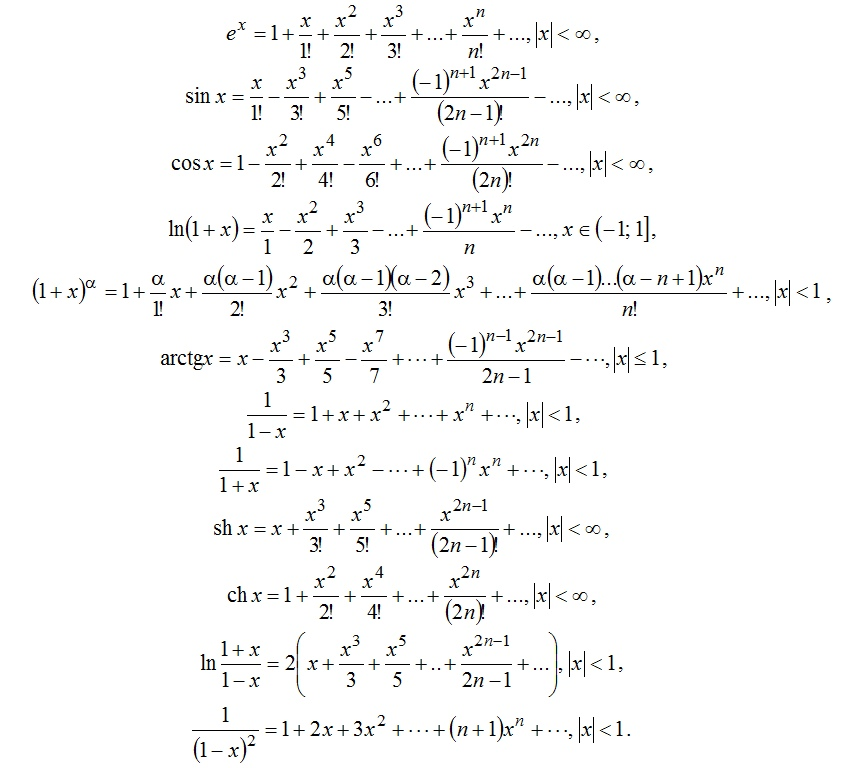
\includegraphics[scale=0.5]{12.jpg}
\end{center}
\newpage
\section{БИЛЕТ 46 -- Правило Лопиталя}
$$ f"X\to\R,\,g:Z\to\R,\,[\,a,b\,]\subset X,\,[\,a,b\,]\subset Z $$
\begin{enumerate}
    \item $$ f(a)=g(a)=0 $$
    \item $$ \exists\,f_{+0}'(a),\:\exists\,g_{+0}'(c)\neq 0,\,c\in Z\:\::\:\lim_{x\to a+0}\frac{f(x)}{g(x)}=\frac{f'(a)}{g'(a)} $$
\end{enumerate}
\newpage
\section{БИЛЕТ 47 -- Исследование функций на монотонность и экстремумы}
Берём производную и ставим знаки
\newpage
\section{БИЛЕТ 48 -- Исследование функций на выпуклость и точки перегиба}
Берём вторую проивзодную и расставляем знаки
\newpage
\section{БИЛЕТ 49 -- Нахождение асимптот графика функции}
Вертикальная асимптота графика, как правило, находится в точке бесконечного разрыва функции. Всё просто: если в точке $x=a$ функция $y=f(x)$ терпит бесконечный разрыв,  то прямая, заданная уравнением $x=a$ является вертикальной асимптотой графика.
\newline
Таким образом, чтобы установить наличие вертикальной асимптоты $x=a$ в точке $x=a$, достаточно показать, что хотя бы один из односторонних пределов $\lim\limits_{x\to a-0}f(x),\,\lim\limits_{x\to a+0} f(x)$ бесконечен. Чаще всего это точка, где знаменатель функции равен нулю.
\newline
\newline
Наклонные (как частный случай – горизонтальные) асимптоты могут нарисоваться, если аргумент функции стремится к $+\infty$ или к $-\infty$. Поэтому график функции не может иметь больше двух наклонных асимптот. Например, график экспоненциальной функции $f(x)=e^x$ обладает единственной горизонтальной асимптотой при $x\to-\infty$, а график арктангенса $f(x)=arctg(x)$ при $x\to-\infty,\,x\to+\infty$ – двумя такими асимптотами, причём различными.
\newline
Нахождение:
\begin{enumerate}
    \item Находим вертикальные асимптоты. Ищем точку, где односторонние пределы бесконечны (предельчики ищем)
    \item Находим наклонные асимптоты. Уравнение вида $y=kx+b$
    $$ k=\lim_{x\to\infty}\frac{f(x)}{x} $$
    $$ b= \lim_{x\to\infty}(f(x)-kx)$$
    Смотри при $+\infty$ и при $-\infty$
\end{enumerate}
\newpage
\section{БИЛЕТ 50 -- Нахождение наибольших и наименьших значений функции}
Находим тчоки минимума или максимума, подставляем их и концы отрезка в функцию, выделяем наименьшее или наибольшее.
\newpage
\end{document}
